\section{Experiment}
\label{sec:experiment}
In this section, we evaluate each step of our approach.
As there is no ground truth for technology comparison, we have to manually check the results of each step or build the ground truth.
And as it is clear to judge whether a tag is of a certain category from its tag description, whether two technologies are comparable, and whether a sentence is a comparative sentence, we recruit two Master students to manually check the results of these three steps.
Only results that they both agree will be regarded as ground truth for computing relevant accuracy metrics, and those results without consensus will be given to the third judge who is a PhD student with more experience.
All three students are majoring in computer science and computer engineering in our school, and they have diverse research and engineering background with different software tools and programming languages in their work.
In addition, we release all experiment data and results in our website\footnote{\url{https://sites.google.com/view/difftech/}}.
 

\subsection{Accuracy of Extracting Comparable Technologies}
This section reports our evaluation of the accuracy of tag category identification, the important of tag category for filtering out irrelevant technologies, and the impact of word embedding models and hyperparameters.

\subsubsection{The Accuracy of Tag Category}
From 33,306 tags with tag category extracted by our method, we randomly sample 1000 tags whose categories are determined using the NLP method, and the other 1000 tags whose categories are determined by the dictionary look-up method (see Section~\ref{sec:categoryKG}).
%As it is clear that whether a tag represents a programming language, a library, or a general computing concept and whether the extracted category corresponds to what a tag represents, 1 final-year Computer Science undergraduate students are recruited to manually examine the category of these 2000 tags by reading their corresponding TagWiki.
%we assign different participants with different sets of tags, so that we can examine as many results as possible with limited number of participants. 
%In this experiment, each participant is assigned 200 tags from the NLP method, and 200 tags from the dictionary look-up method for checking.
Among the 1000 sampled tag categories by the NLP method, categories of 838 (83.8\%) tags are correctly extracted by the proposed method.
For the 1000 sampled tags by the dictionary look-up method, categories of 788 (78.8\%) tags are correct.

According to our observation, two reasons lead to the erroneous tag categories.
First, some tag definition sentences are complex which can lead to erroneous POS tagging results.
For example, the tagWiki of the tag \textit{rpy2} states that ``RPy is a very simple, yet robust, Python interface to the R Programming Language''. 
The default POS tagging	recognizes \textit{simple} as the noun which is then regarded as the category by our method.
Second, the dictionary look-up method sometimes makes mistakes, as the matched category may not be the real category.
For example, the TagWiki of the tag \textit{honeypot} states ``A trap set to detect or deflect attempts to hack a site or system''.
Our approach matches the \textit{system} as the category of the \textit{honeypot}.

\subsubsection{The Importance of Tag Category}
To check the importance of tag category for the accurate comparable technology extraction, we set up two methods, i.e., one is word embedding and tag category filtering, and the other is only with word embedding.
The word embedding model in two methods are both skip-gram model with the word embedding dimension as 800.  
We randomly sample 150 technologies pairs extracted from each method, and manually check the if the extracted technology pair is comparable or not.
It shows that the performance of model with tag category (90.7\%) is much better than that without the tag category filtering (29.3\%).

\subsubsection{The impact of parameters of word embedding}
%The are two kinds of widely-used word embedding models, the skip-gram model and CBOW model mentioned in Section~\ref{sec:w2v}.
\label{sec:comparison_w2v}
There are two important parameters for the word embedding model, and we test its impact on the the performance of our method.
First, we compare the performance of CBOW and Skip-gram mentioned in Section~\ref{sec:w2v} by randomly sampling 150 technology pairs extracted by each method under the same parameter setting (the word embedding dimension is 400).
The results show that Skip-gram model (90.7\%) outperforms the CBOW model (88.7\%), but the difference is marginal.

Second, we randomly sample 150 technologies pairs by the skip-gram model with different word embedding dimensions, and manually check the accuracy.
From the dimension 200 to 1000 with the step as 200, the accuracy is 70.7\%, 72.7\%, 81.3\%, 90.7\%, 87.3\%.
We can see that the model with the word embedding dimension as 800 achieves the best performance.
Finally, we take the Skip-gram model with 800 word-embedding dimension as the word embedding model to obtain the comparable technologies in this work.   

\subsection{Accuracy and coverage of comparative sentences}
We evaluate the accuracy and coverage of our approach in finding comparative sentences from the corpus.
\wang{We first randomly sample 350 sentences (50 sentences for each comparative sentence pattern in Table~\ref{tab:patternSingle} and Table~\ref{tab:patternMultiple}) which are extracted by our model.
We manually check the accuracy of the sampled sentences and Table~\ref{tab:patternAccuracy} shows the results.
The overall accuracy of comparative sentence extraction is 89.1\%, and our approach is especially accurate for the first 2 patterns for single sentence and all three patterns for contextual sentences.
The last two patterns for single sentence do not get good performance due to the relatively loose conditions.}

\wang{
We further check the wrong extraction of comparative sentences and find that most errors from single sentence patterns are caused when the two comparative technologies are listed together for a similar feature, i.e. ``\textit{Java framework awt or swing makes more sense for something this simple}''} or when the two comparative technologies are used to compare with a third technology like ``\textit{I mean it came as a surprise to me that drupal is so much faster than wordpress and joomla}''.
In addition, although some sentences do not contain the question mark, they are actually interrogative sentence such as ``\textit{I also wonder if postgresql will be a win over mysql}''.
\wang{
For contextual sentences, we also find out that sometimes the sentence is comparing the two selected technology pairs with a third one. And sometimes for the AFF-NEG pattern, it seems although both sentences mentioned two comparative technologies respectively, they aren't tended to compare them, i.e. ``\textit{Vim does only text editing and that very well without plugins.
Its up to you if you like emacs or not.}''}
%Second, the comparison between the two similar technologies is quantitive (e.g., a \textit{ng-app} can have more than one \textit{ng-controller}).

\begin{comment}
\begin{figure}
	\centering
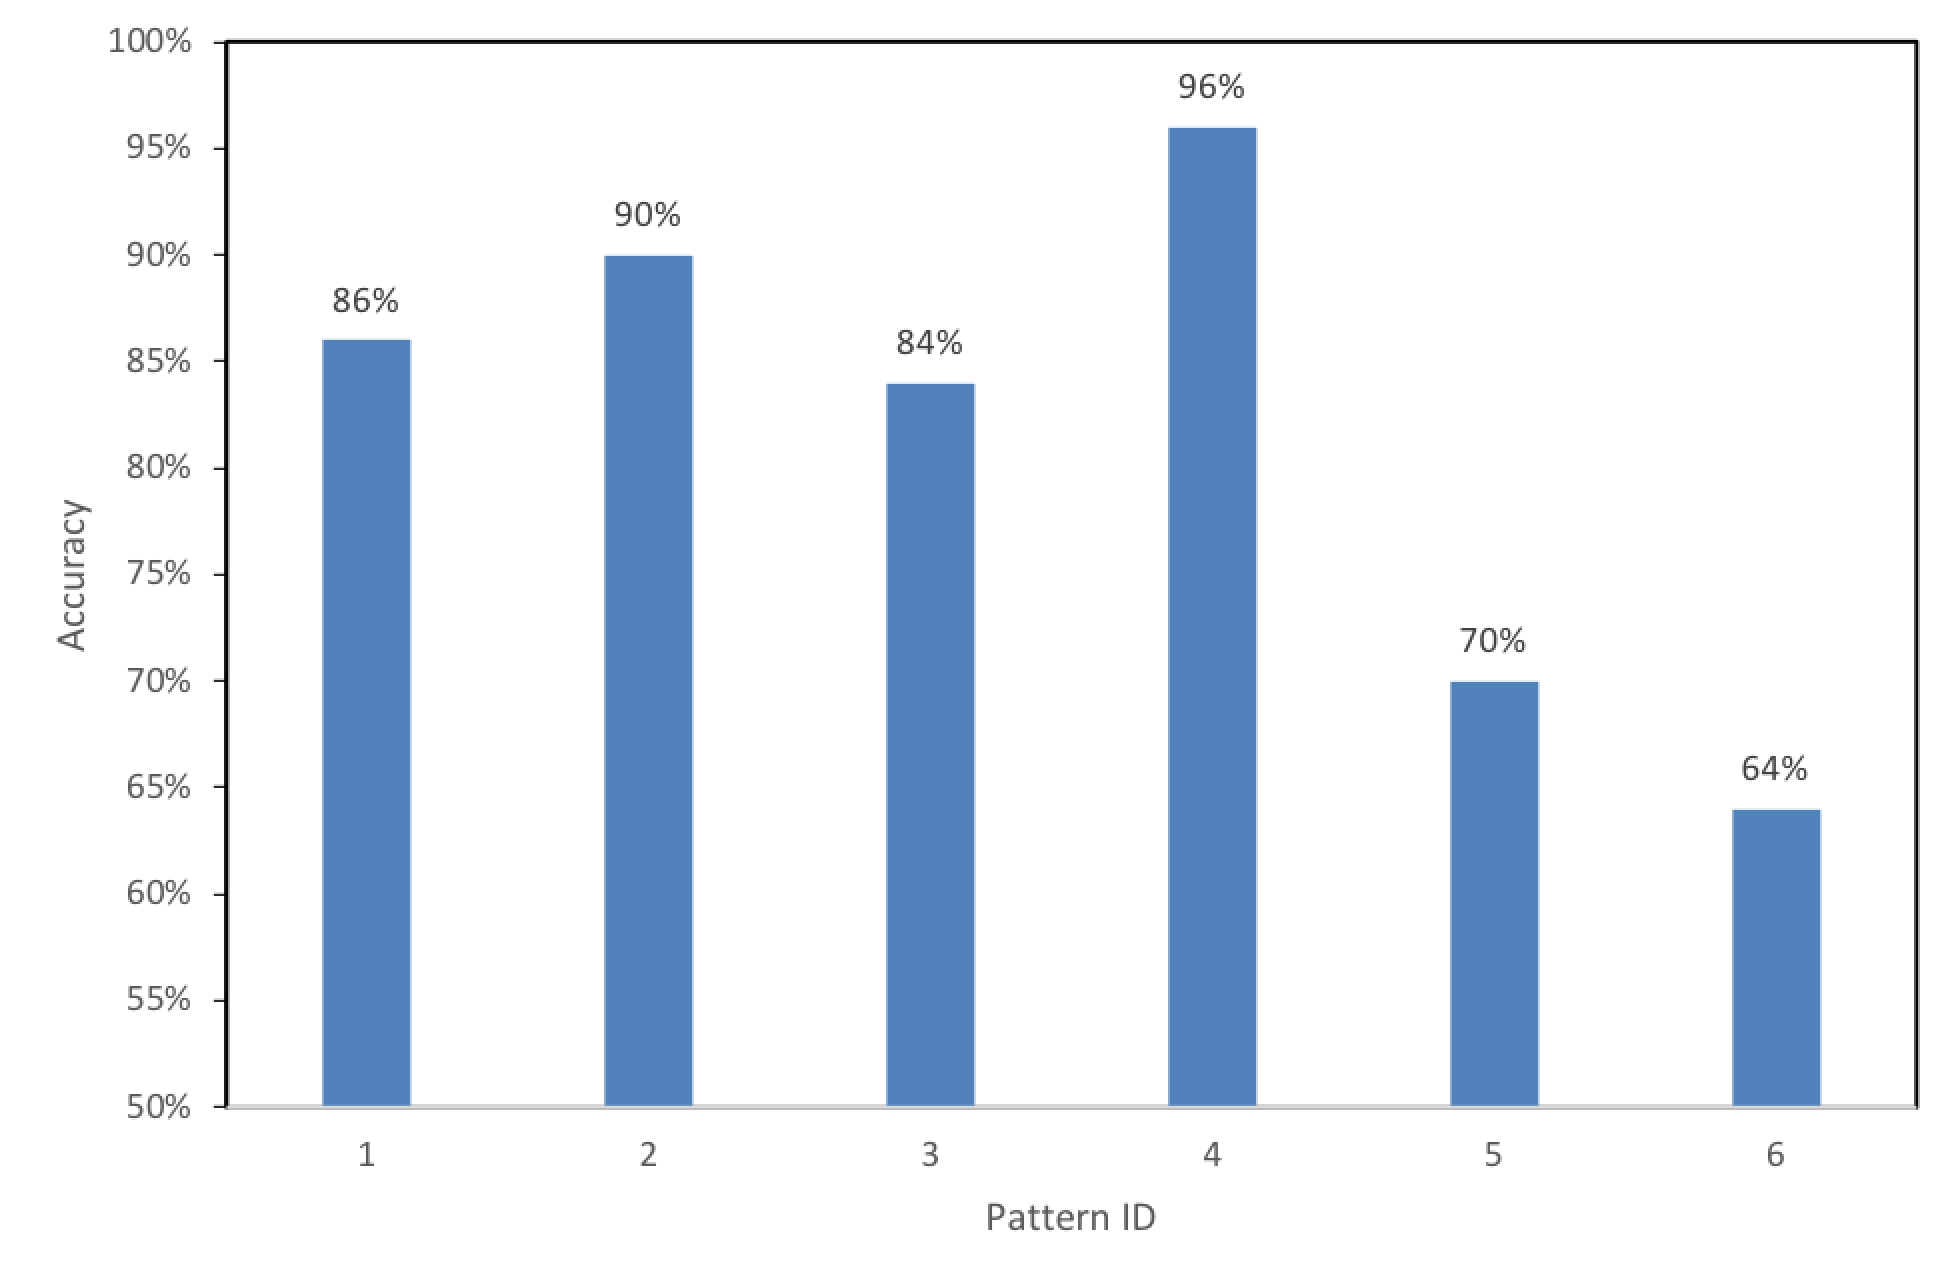
\includegraphics[width=0.5\textwidth]{figures/patternAccuracy.png}
	\label{fig:patternAccuracy}
\end{figure}	
\end{comment}


\begin{table}
	\centering
	\caption{The accuracy of comparative sentences extraction}
	\vspace{-2mm}
	\begin{tabular}{c c c c c}
	\hline
	\multicolumn{5}{c}{Single sentence}\\
	\hline
	\textbf{No.} & Pattern & \textbf{\#right} & \textbf{\#wrong} & \textbf{Accuracy} \\ \hline
	1 & \textit{TECH * VBZ * JJR/RBR} & 47 & 3  & 94\% \\
	2 & \textit{(RBR JJ) /JJR * CIN * TECH} & 46 & 4  & 92\% \\
	3 & \textit{CV * CIN TECH} & 42 & 8 & 82\% \\
	4 & \textit{CV VBG TECH} & 38 & 12 & 76\% \\
	\hline
	\multicolumn{5}{c}{Contextual sentences}\\
	\hline
	\textbf{No.} & Pattern & \textbf{\#right} & \textbf{\#wrong} & \textbf{Accuracy} \\ \hline
	1 & \textit{TECH * VBZ * JJR/RBR} & 47 & 3  & 94\% \\
	2 & \textit{(RBR JJ) /JJR * CIN * TECH} & 47 & 3  & 94\% \\
	3 & \textit{AFF-NEG} & 45 & 5  & 90\% \\
	\hline
	Total &  & 312 & 38 & 89.1\% \\
	\hline
	\end{tabular}
	\vspace{-2mm}
	\label{tab:patternAccuracy}
\end{table}

\begin{comment}
To measure the coverage, we first find all sentences that contain pairs of similar technologies.
Then we randomly sample 200 sentences of them, and find \textcolor{red}{??} sentences are comparative sentences via the manual check.
Among \textcolor{red}{??} comparative sentences, \textcolor{red}{?? (??\%) of them are successfully extracted by our approach.}
\textcolor{red}{For the ?? comparative sentences we missed, we conclude xx reasons: 1) 2) CCY: Please tell why we cannot find some of them.}
%For coverage, we compare the baseline without using synonyms and abbreviations in our previous work~\cite{chen2017unsupervised}.
\end{comment}

\subsection{Accuracy of clustering comparative sentences}
\label{sec:clusterEvaluate}
We evaluate the performance of our opinion clustering method by comparing it with the baseline methods.

\subsubsection{Baseline}
\wang{
We set up three baselines to compare with our comparative sentence clustering method. 
The first baseline is the traditional TF-IDF~\cite{sparck1972statistical} with K-means~\cite{hartigan1979algorithm}, the second baseline is based on the document-to-vector deep learning model (i.e., Doc2vec~\cite{le2014distributed}) with K-means, and the last one is BERT~\cite{devlin2018bert} with K-means.
All of methods first convert the comparative sentences for a pair of comparable technologies into a list of vectors.
%We train both models with all comparative sentences in our corpus.
Then, we carry out K-means algorithms to cluster the sentence vectors into $N$ clusters.
To make the baseline as competitive as possible, we set $N$ at the cluster number of the ground truth.
In contrast, our method specifies its cluster number by community detection which may differ from the cluster number of the ground truth.}
\chen{Will check this paragraph later.}

\subsubsection{Ground Truth}
\label{sec:clusteringGroundTruth}
As there is no ground truth for clustering comparative sentences, we ask two Master students mentioned before to manually build a small-scale ground truth.
We randomly sample 15 pairs of comparable technologies with different number of comparative sentences.
For each technology pair, the two students read each comparative sentence and each of them will individually create several clusters for these comparative sentences.
Note some comparative sentences are unique without any similar comparative sentence, and we put all those sentences into one cluster.
Then they will discuss with the Ph.D student about the clustering results, and change the clusters accordingly.
Finally, they reach an agreement for 10 pairs of comparable technologies.
We take these 10 pairs as the ground truth whose details can be seen in Table~\ref{tab:groundTruth}.

\begin{table}
	\centering
	\small
	\caption{Ground truth for evaluating clustering results}
	\vspace{-2mm}
	\setlength{\tabcolsep}{0.01em}
	\begin{tabular}{c c c c}
	\hline
	\textbf{No.} & \textbf{Technology pair} & \textbf{\#comparative sentence} & \textbf{\#cluster} \\ \hline
	1 & \textit{compiled \& interpreted language} & 34 & 4 \\
    2 & \textit{sortedlist \& sorteddictionary} & 18 & 4 \\
	3 & \textit{quicksort \& heapsort} & 51 & 5 \\
	4 & \textit{ant \& maven} & 83 & 9 \\
	5 & \textit{lxml \& beautifulsoup} & 52 & 6 \\
	6 & \textit{awt \& swing} & 53 & 7 \\
	7 & \textit{jackson \& gson} & 39 & 3 \\
	8 & \textit{jruby \& mri} & 25 & 4 \\
	9 & \textit{pypy \& cpython} & 72 & 7 \\
	10 & \textit{memmove \& memcpy} & 33 & 3 \\
	\hline
	\end{tabular}
	\vspace{-3mm}
	\label{tab:groundTruth}
\end{table}

\subsubsection{Evaluation Metrics}
\label{sec:clusteringGroundTruth}
Given the ground truth clusters, many metrics have been proposed to evaluate the clustering performance in the literature.
In this work, we take the Adjusted Rand Index (ARI)~\cite{hubert1985comparing}, Normalized Mutual Information(NMI)~\cite{vinh2010information}, homogeneity, completeness, V-measure~\cite{rosenberg2007v}, and Fowlkes-Mallows Index (FMI)~\cite{fowlkes1983method}.
For all six metrics, higher value represents better clustering performance.
For each pair of comparable technologies, we take all comparative sentences as a fixed list, and $G$ as a ground truth cluster assignment and $C$ as the algorithm clustering assignment.

\textbf{Adjusted Rand Index (ARI)} measures the similarity between
two partitions in a statistical way.
It first calculates the raw Rand Index (RI) by $ RI = \frac{a+b}{C^{N}_{2}}$ where $a$ is the number of pairs of elements that are in the same cluster in $G$ and also in the same cluster in $C$, and $b$ is the number of pairs of elements that are in different clusters in $G$ and also in different clusters in $C$.
$C^{N}_{2}$is the total number of possible pairs in the dataset (without ordering) where $N$ is the number of comparative sentences.
To guarantee that random label assignments will get a value close to zero, ARI is defined as 
$$ ARI = \frac{RI - E[RI]}{\max (RI) - E[RI]}$$
where $E[RI]$ is the expected value of $RI$.

\textbf{Normalized Mutual Information (NMI)} measures the mutual information between the ground truth labels $G$ and the algorithm clustering labels $C$, followed by a normalization operation:
$$ NMI(G, C) = \frac{MI(G, C)}{\sqrt{H(G) H(C)}} $$
where $H(G)$ is the entropy of set $G$ i.e., $H(G) = - \sum^{|G|}_{i=1}P(i) \log (P(i)) $ and $P(i) = \frac{G_i}{N}$ is the probability than an objet picked at random falls into class $G_i$.
The $MI(G, C)$ is the mutual information between $G$ and $C$ where $MI(G, C) = \sum^{|G|}_{i=1} \sum^{|C|}_{j=1} P(i, j) \log ( \frac{P(i, j)}{P(i)P(j)} )$


\textbf{Homogeneity (HOM)} is the proportion of clusters containing only members of a single class by
$$ h = 1 - \frac{H(G|C)}{H(G)} $$
\textbf{Completeness (COM)} is the proportion of all members of a given class are assigned to the same cluster by
$$ c = 1 - \frac{H(C|G)}{H(C)} $$
where $H(G|C)$ is the conditional entropy of the ground-truth classes given the algorithm clustering assignments.

\textbf{V-measure (V-M)} is the harmonic mean of homogeneity and completeness
$$ v = 2 \times \frac{h\times c}{h+c} $$

\textbf{Fowlkes-Mallows Index (FMI)} is defined as the geometric mean of the pairwise precision and recall:
$$ FMI = \frac{TP}{\sqrt{(TP+FP)(TP+FN)}} $$
where $TP$ is the number of True Positive (i.e. the number of pairs of comparative sentences that belong to the same clusters in both the ground truth and the algorithm prediction), $FP$ is the number of False Positive (i.e. the number of pairs of comparative sentences that belong to the same clusters in the ground-truth labels but not in the algorithm prediction) and $FN$ is the number of False Negative (i.e the number of pairs of comparative sentences that belongs in the same clusters in the algorithm prediction but not in the ground truth labels).

\subsubsection{Overall Performance}
\wang{
Table~\ref{tab:clusterEvaluation} shows the evaluation results.
the three baseline methods has similar results whereas tf-idf and Sentence-Bert are slitly better, but our model significantly outperforms all models in all six metrics.}

According to our inspection of detailed results, we find two reasons why our model outperforms the baselines.
First, our model can capture the semantic meaning of comparative sentences.
TF-IDF can only find similar sentences using the same words but count similar words like ``secure'' and ``safe'' as unrelated.
While the sentence vector from Doc2vec is easily influenced by the noise as it takes all words in the sentence into consideration. \wang{The Bert model would break word that it doesn't recognised into pieces, i.e.heapsort to heap-, -sort. In this way they might conduct vectors that is not close to the original words. Also, the BERT model is trained by general corpus(like wikipeidia), which is different from our technology-specific dataset.}
Second, constructing the similar sentences as a graph in our model explicitly encodes the sentence relationships.
The community detection based on the graph can then easily put similar sentences into clusters.
In contrast, for the four baselines, the error brought from them is accumulated and amplified to K-means in the clustering phase.

\begin{table}
	\centering
	\caption{Clustering performance}
	\vspace{-2mm}
	\setlength{\tabcolsep}{0.5em}
	\begin{tabular}{lllllll}
	\hline
	\textbf{Method} & \textbf{ARI} & \textbf{NMI} & \textbf{HOM} & \textbf{COM} & \textbf{V-M} & \textbf{FMI} \\ \hline
	TF-IDF+Kmeans  & 0.09&0.24&0.35&0.28&0.26&0.25\\
	Doc2vec+Kmeans & 0.01&0.17&0.29&0.20&0.18&0.18\\
	%BERT+Kmeans & 0.01&0.18&0.31&0.20&0.19&0.18\\
	Bert+Kmeans & 0.10&0.24&0.35&0.28&0.26&0.26\\
	\tool & \textbf{0.65}&\textbf{0.67}&\textbf{0.76}&\textbf{0.77}&\textbf{0.72}&\textbf{0.71}\\
	\hline
	\end{tabular}
	\vspace{-1mm}
	\label{tab:clusterEvaluation}
\end{table}

\subsection{Accuracy of Opinion Summarization}
\label{sec:summarization}
\wang{All of this section are newly added}
\chen{Please add more details in this section}
In this section, we evaluate the accuracy of our overall opinion summarization. We compare our methods with five different baselines that are commonly used in sentence analysis. We implement those baselines and use four metrics to compare them with our methods, and our methods performs better in opinion summarization than the rest of them.

\subsubsection{Baselines}
\chen{Where is FastText?}
In this section, we set up five baselines to compare with our method. The first baseline is TF-IDF\cite{sparck1972statistical} with SVM \cite{Cortes1995}, whereas the second one is N-gram vectorizer with SVM. The two models firstly covert the train sentences into vectors. Then, we use the Support Vector Machines(SVM) to make predictions for the given sentences. For both of the models, we tried to use different size of C in SVM in order to avoid the misclassifying of the vectors. Then, we also build another two baselines which are Convolutional Neural Network(CNN) and Long Short Term Memory(LSTM). Both of them are neural networks that can be trained for classification after text embedding. The last baseline is FastText~\cite{joulin2016fasttext}, which is a pre-trained model released by Facebook for text classification and representation learning.
\begin{table}
	\scriptsize
	\center	
	\caption{Examples of labeled sentences \chen{1) Please replace the first example, and it can be regarded as a wrong case, 2)Please give one example for each case 3) Please use label ``support A'', ``neutral'' as the name.}}
	\vspace{-4mm}
	%\setlength{\tabcolsep}{0.3em}
	\begin{tabular}{c |l}
		\hline
		\textbf{Label} & \textbf{Sentence} \\
		\hline
        \multirow{1}{*}{Neutral} & I am not sure if TechA server will be much better than TechB\\
        \hline
        \multirow{1}{*}{Support Tech A} & I do know TechA better than TechB\\
        \hline
        \multirow{1}{*}{Support Tech B} & Also have a look at TechB which is safer version of TechA\\
				\hline
	\end{tabular}
	\vspace{-3mm}
	\label{tab:label}
\end{table}
\subsubsection{Dataset}
\revise{As we are adopting the supervised model for opinion summarization, we manually create a set of labels annotating which technology does the sentence support.
We randomly select 801 and 150 comparative sentences as the training and testing datasets respectively. 
We replace the comparable technology pairs with two unique tokens i.e., TechA (first occurrence) and TechB (second occurrence) to generalize different technology pairs.
For each sentence, two authors in this paper label it as one of three categories including supporting TechA, supporting TechB, or neutral, shown in Table~\ref{tab:label}
Note that the two annotators work individually and the sentence can be taken in to the consideration only when they reach the agreement.
There are more sentences about supporting TechA or TechB, but fewer neutral sentences.
To balance the data from three categories, we remove some comparative sentences about supporting certain technology, with 267 sentences for supporting TechA, 267 for supporting TechB and 267 neutral ones.
}
 
%From all the comparative sentences, we randomly sample 800 sentences as training set. Then, we randomly sample another 150 sentences as testing set. Then, as being mentioned in Section~\ref{{sec:fineTuning}}, we label both the training set and the testing set with 0,1,2 based on the semantic meaning of sentences. Then we leverage the 800 sentences training set to 817 sentences which including 275 \textit{label 0} sentences, 275 \textit{label 1} sentences, and 267 \textit{label 2} sentences, so that the number of each type of sentences are relatively equal.

\subsubsection{Metrics} 
\revise{
As this is a typical multi-class classification task, we adopt four metrics for measuring the performance of our model including accuracy, precision, recall, and F1-score. 
%as metrics to evaluate the accuracy of our opinion summarization. 
All of these metrics are based on the four statistics: TP (true positive) represents the number of sentences that are correctly classified as one label; 
TN (true negative) represents the number of sentences that are corrected classified as not that label; 
FP (false positive) represents the number of sentences that are predicted as the label, but the it's not;
FN (false negative) represents the number of sentences that as not the label, but actually it is in the label;
}

\textbf{Accuracy} is the proportion of correct result among the whole test case: 
$ Accuracy = \frac{TP+TN}{(TP+FP+TN+FN)} $

\textbf{Precision} is the ratio of the correctly predicted positive records to the whole positive records:
$ Precision = \frac{TP}{(TP+FP)} $

\textbf{Recall} is calculating the correctly predicted positive records among all predicted positive records:
$ Recall = \frac{TP}{(TP+FN)} $

\textbf{F1-score}  is the harmonic mean of precision and recall, which can combine both of the two metrics above:
$ F1-score = 2*\frac{Precision*Recall}{(Precision+Recall)} $

\revise{
Note that these metrics are default for binary classification.
As our task is a multi-class classification, we adopt the macro average~\cite{web:macroAverage} of these metrics for each class as the overall performance for this model.
%calculate the four scores for each label independently (i.e whe n calculate label 0, all sentences with label 0 are positive and rest of them are negative). Then we take the metrics from three labels and calculate the macro average of four metrics and have the final results.
A higher value represents better performance for all the metrics.
%\chen{There are two kinds of average, micro and macro, and can you do both of them?}
}

\subsubsection{Overall Performance}
\chen{One paragraph is needed to analyze why other models do not work well, and another paragraph for analyzing the reasons of our wrong cases?}
Table~\ref{tab:opinionSummarizationPerformance} shows the experiment results. We can see that TF-IDF with SVM has the worst performance, CNN and LSTM have similar performance which are both better than TF-IDF, FastText is slightly better than them, and n-gram with SVM has the highest among other baselines. Our model performs the best out of the five methods. \wang{TF-IDF has the worst performance is probably because it can't capture the semantic information of complex sentences. For CNN, LSTM, and FastText the problem could be the size of our training corpus is not large enough. N-gram with SVM model performs good is because it takes a sequence words together, so that the model can read the sentence semantics better.}
We think the reason our model performs the best is that we use BERT. It offers sentence level classification, and has been trained with large data corpus. It results in a better performance when dealing with such sentiment analysis problems.

\begin{table}
	\centering
	\caption{Opinion summarization performance \chen{Please use decimals within 0 to 1}}
	\vspace{-2mm}
	\setlength{\tabcolsep}{0.5em}
	\begin{tabular}{lllll}
	\hline
	\textbf{Method} & \textbf{accuracy} & \textbf{precision} & \textbf{recall} & \textbf{f1-score} \\ \hline
	TF-IDF+SVM  & 0.533 & 0.506 & 0.513 & 0.507 \\
	n-gram+SVM &  0.753 & 0.741 & 0.749 & 0.741\\
	CNN & 0.62& 0.573 & 0.585 &0.57\\
	LSTM & 0.633 & 0.613 & 0.622 & 0.614\\
	FastText & 0.68 & 0.658 & 0.663 & 0.659\\
	\tool & \textbf{0.847} & \textbf{0.843} & \textbf{0.854} & \textbf{0.841}\\
	\hline
	\end{tabular}
	\vspace{-1mm}
	\label{tab:opinionSummarizationPerformance}
\end{table}

\revise{Despite good performance of our model, there are still some wrong cases within our model.
We manually check those wrongly predicted sentences, and find that most wrong predictions are caused by the neutral ones.
For example, our model make mistake in the sentence ``I am not sure if VMware Server will be much better than VirtualBox.'' into supporting VMware.
The sentence structure may be too complicated for the BERT model, but more labeled dataset in the future may help mitigate that effect. And some of the wrong predicted cases are the sentence is comparing two technologies, but they are not expressing their feelings on which they prefer, but focus on how different they are. For example in the sentence ``char is guaranteed to be smaller than int'' is simply indicate that char type takes less storage space than int type, it's a neutral express, but our model would take it into support int.}
%  \chen{Please replace TechA, TechB with the real examples, and add more analysis of wrong predictions.}}
 
 \subsection{Experiments on Generality}
\wang{Besides the Stack Overflow site, we also carry out our method to other Stack Exchange Sites, like Super User and Unix and Linux. Just like Stack Overflow, both of the sites are Q\&A sites, but they focus on different perspectives. For the experiments, we also use the dataset released on 4 September 2019. }

\wang{After conduct our methods to those two datasets, we randomly sampled 50 comparative sentences from each site. From the Table \ref{tab:generality} we can see that both of the website have an accuracy over 80\%. Based on the experiments we can say that our method construct domain-specific thesaurus, showing that our method has the generality for most of the Q\&A websites.}

\begin{table}
	\centering
	\caption{The accuracy of comparative sentences extraction}
	\vspace{-2mm}
	\begin{tabular}{c c c c}
	\hline
	Source & \textbf{\#right} & \textbf{\#wrong} & \textbf{Accuracy} \\ \hline
	Unix and Linux & 44 & 6  & 88\% \\
	Super User & 42 & 8  & 82\% \\
	\hline
	\end{tabular}
	\vspace{-2mm}
	\label{tab:generality}
\end{table}